\documentclass[11pt]{article}
\usepackage{graphicx}
\usepackage[T1]{fontenc}
\usepackage[polish]{babel}
\usepackage{tabularx}
\usepackage[table,xcdraw]{xcolor}
\usepackage[utf8]{inputenc}
\usepackage{lmodern}
\usepackage{multirow}
\usepackage{array}
\usepackage{booktabs}
\selectlanguage{polish}
\usepackage{titlesec}
\usepackage{amsmath}
\usepackage{esint}
\usepackage{textpos}
\usepackage{chngpage}
\usepackage{calc}
\usepackage{algorithm}
\usepackage[noend]{algpseudocode}
\usepackage{placeins}
\usepackage{longtable}

\let\Oldsection\section
\renewcommand{\section}{\FloatBarrier\Oldsection}

\let\Oldsubsection\subsection
\renewcommand{\subsection}{\FloatBarrier\Oldsubsection}

\let\Oldsubsubsection\subsubsection
\renewcommand{\subsubsection}{\FloatBarrier\Oldsubsubsection}
\titlelabel{\thetitle.\quad}

\begin{document}
\begin{titlepage}
\centering

{\large Wydział Matematyki i Nauk Informacyjnych Politechniki Warszawskiej}

\vspace{1cm}

\includegraphics[scale=0.15]{logo}
\vspace{3cm}

{\Huge\bfseries Symulacja wyścigów samochodowych w 3D}

\vspace{0.5cm}

{\Large Grafika Komputerowa I}
\vspace{2cm}

{\Large Autor: \textbf{Maciej Grzeszczak}}

\vspace{1cm}

{\large v1.1}

\vspace{1cm}

\vfill

{\itshape {\large 10 grudnia 2016r.}}
\end{titlepage}

\tableofcontents


\begin{table}[!h]
\centering
\def\arraystretch{2}%
\caption{Lista zmian}

\resizebox{\textwidth}{!}{
\begin{tabular}{|p{3cm}|p{4cm}|p{6cm}|p{2cm}|}
\hline
Data                 & Autor             & Opis zmiany                                                               & Wersja                                                 \\ \hline
17.12.2016                      & Maciej Grzeszczak      & Opis architektury oraz rozwinięcie opisu biznesowego  & 1.1 \\ \hline
10.12.2016                      & Maciej Grzeszczak      & Pierwsza wersja dokumentu  & 1.0 \\ \hline
                      
\end{tabular}%
}
\end{table}


\newpage


\section{Specyfikacja}
\subsection{Opis biznesowy}

\par Niniejszy program to aplikacja przeglądarkowa, wykorzystująca technologię WebGL w postaci biblioteki three.js. Będzie ona zoptymalizowana głównie pod przeglądarkę Mozilla Firefox. 
\par Aplikacja jest symulacją wyścigów samochodowych w 3D. Umożliwia użytkownikowi prowadzenie pojazdu za pomocą odpowiednich klawiszy i ściganie się z samochodami sterowanymi przez komputer. Dany będzie jeden, z góry określony tor po którym będzie można jeździć, sam gracz będzie mógł również go opuścić i poruszać się po całej mapie. Samochód będzie przyspieszał, hamował i skręcał w zależności od wciśniętych klawiszy, będzie można również włączyć bieg wsteczny. 
\par Aplikacja służy również jako pokaz różnych modeli oświetlenia oraz cieniowania. Gracz będzie mógł za pomocą odpowiednich przycisków zmienić obecny model oświetlenia na model Phonga lub Blinna, jak również wybrać jeden z trzech trybów cieniowania (Phonga, Gourauda, stałe). 
\par Oprócz tego, dostępne będą cztery kamery, umożliwiające obserwowanie wyścigów z różnych perspektyw, między innymi ze środka kabiny oraz zza pojazdu, która będzie płynnie poruszać się z pojadem, wykorzystując do tego interpolację.
\par W planach jest również wprowadzenie większej ilości torów, możliwości ich wczytywania z tekstur, wprowadzenie nierówności terenu i dostosowywania się auta do nich, oraz użycie oddzielnych modeli do kół pojazdów, co umożliwiłoby ich kręcenie się oraz skręcanie.
\subsection{Wymagania funkcjonalne}
Poniższy rysunek w postaci diagramu UML przedstawia możliwe przypadki użycia systemu przez użytkownika:
\\
\\
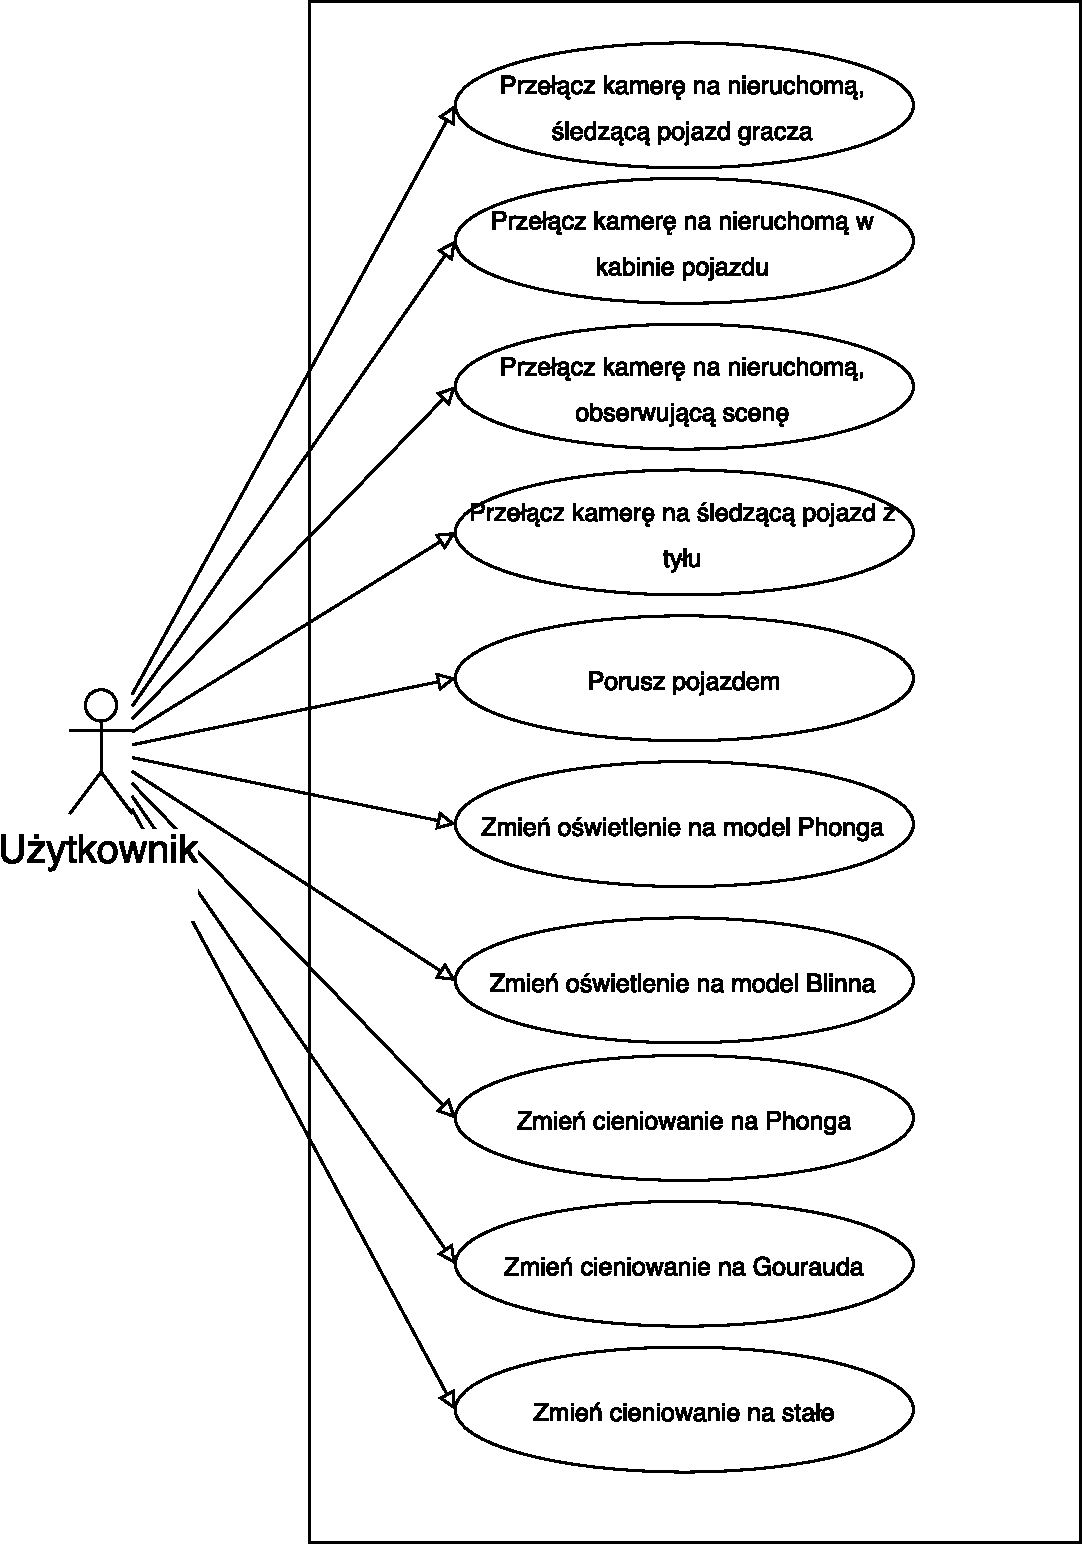
\includegraphics[scale=0.5]{use_case_pdf}

\begin{table}[!h]
\centering
\def\arraystretch{2}%
\caption{Opisy przypadków użycia dla użytkownika}

\resizebox{\textwidth}{!}{
\begin{tabular}{|p{2cm}|p{3cm}|p{6cm}|p{6cm}|}
\hline
Aktor                 & Nazwa             & Opis                                                               & Odpowiedź systemu                                                 \\ \hline
\multirow{7}{*}{Użytkownik} & Przełącz kamerę na nieruchomą, z kabiny pojazdu.   & Zmiana położenia kamery na kabinę pojazdu, skierowaną na drogę przed pojazdem. & Natychmiastowa zmiana pozycji kamery.            \\ \cline{2-4} 
                      & Przełącz kamerę na nieruchomą, obserwującą całą scenę.       & Zmiana położenia kamery na pozycję umożliwiającą obserwowanie całej sceny z oddali.  & Natychmiastowa zmiana pozycji kamery. \\ \cline{2-4}
                      & Przełącz kamerę na nieruchomą, śledzącą pojazd gracza.       & Zmiana położenia kamery na pozycję, która jest nieruchoma i śledzi pojazd gracza.  & Natychmiastowa zmiana pozycji kamery. \\ \cline{2-4}
                      & Przełącz kamerę na śledzącą pojazd z tyłu.       & Zmiana położenia kamery na pozycję za pojazdem, która porusza się za pojazdem płynnie i wykorzystuje do tego interpolację  & Natychmiastowa zmiana pozycji kamery. \\ \cline{2-4}
                      & Porusz pojazdem.       & Przemieszczenie się pojazdu pod wpływem wciśnięcia odpowiednich klawiszy.  & Przemieszczenie się pojazdu. \\ \cline{2-4}                                            
                      & Zmień oświetlenie na model Phonga.       & Zmiana obecnego modelu oświetlenia na model Phonga.  & Natychmiastowa zmiana modelu oświetlenia na model Phonga. \\ \cline{2-4}
                      & Zmień oświetlenie na model Blinna.       & Zmiana obecnego modelu oświetlenia na model Blinna.  & Natychmiastowa zmiana modelu oświetlenia na model Blinna. \\ \cline{2-4}
					 & Zmień cieniowanie na Phonga.       & Zmiana obecnego trybu cieniowania na cieniowanie Phonga.  & Natychmiastowa zmiana trybu cieniowania na cieniowanie Phonga. \\ \cline{2-4}
					& Zmień cieniowanie na Gourauda.       & Zmiana obecnego trybu cieniowania na cieniowanie Gourauda.  & 	Natychmiastowa zmiana trybu cieniowania na cieniowanie Gourauda. \\ \cline{2-4}
					& Zmień cieniowanie na stałe.       & Zmiana obecnego trybu cieniowania na stałe.  & Natychmiastowa zmiana trybu cieniowania na cieniowanie stałe. \\ \hline
                      
\end{tabular}%
}
\end{table}



\subsection{Wymagania niefunkcjonalne}
Poniżej przykładowe wymagania niefunkcjonalne pogrupowane w poszczególne kategorie URPS.


\begin{center}

\begin{table}[!h]
\centering
\def\arraystretch{2}%
\caption{Lista wymagań niefunkcjonalnych}
\label{my-label}
\resizebox{\textwidth}{!}{
\begin{tabular}{|p{3cm}|p{0.5cm}|p{10cm}|}
\hline
Obszar wymagań &Lp & Opis                                                                                         \\ \hline
\multirow{1}{*}{Użyteczność}    & 1               & Aplikacja będzie działała na przeglądarce Mozilla Firefox dla każdej rozdzielczości powyżej 800x600. \\ \hline
\multirow{1}{*}{Niezawodność}   & 2               & Aplikacja będzie dostępna 24/7 pod podanym adresem. \\ \hline
\multirow{2}{*}{Wydajność}      
& 3               & Aplikacja będzie utrzymywać minimalny poziom 15 FPS (klatek na sekundę).  \\ \hline
\multirow{1}{*}{Utrzymanie}     
& 4               & Wraz z aplikacją zostaje dostarczona instrukcja użytkownika. \\ \hline
\end{tabular}
}
\end{table}
\end{center}

\subsection{Harmonogram projektu}

%\includegraphics[scale=0.45]{harmonogram}
%\\
%\par \noindent
\par Implementacja projektu zostanie podzielona na dwie fazy:
\begin{enumerate}
\item \textbf{Faza tworzenia sceny (14 dni)} - stworzenie świata wraz z obiektami (pojazdami), implementacja poruszania się pojazdem oraz poruszania się i zmiany pozycji kamery.
\item \textbf{Faza implementacji poszczególnych modelów oświetlenia oraz cieniowania (7 dni)} - implementacja modeli oświetlenia Phonga i Blinna oraz cieniowań: stałego, Phonga i Gourauda.
\end{enumerate}
\par \noindent

\newpage
\subsection{Architektura rozwiązania}
\begin{center}
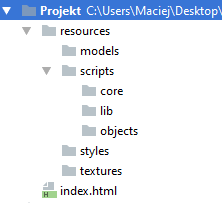
\includegraphics[scale=1]{architecture}
\end{center}

Powyższe zdjęcie przedstawia szkielet architektury projektu. Poniżej znajduje się opis kolejnych elementów.

\begin{enumerate}
\item \textbf{index.html} - główny i jedyny plik html, w którym zagnieżdżony będzie HTML5 Canvas.
\item \textbf{resources} - folder, w którym znajdują się wszystkie zasoby wykorzystywane przez aplikację:
\begin{enumerate}
\item models - folder z modelami 3D używanymi przez aplikację
\item scripts - folder ze skryptami Javascript
\begin{enumerate}
\item core - folder zawierający pliki .js dotyczące szkieletu działania aplikacji, czyli pętli gry, liczenia fizyki, renderowania, obsługiwania interakcji użytkownika.
\item objects - folder w którym znajdują się pliki .js definiujące wszystkie obiekty wykorzystywane w aplikacji, między innymi pojazdu, kamery, mapy.
\item lib - folder w którym znajdują się pliki .js zewnętrznych bibliotek.
\end{enumerate}
\item styles - folder z wszystkimi plikami .css
\item textures - folder z teksturami wykorzystywanymi przez aplikację
\end{enumerate}
\end{enumerate}

Oprócz tego projekt będzie oparty na wzorcu modułów, który pomaga w organizacji całości kodu oraz uzyskania tzw. 'loose coupling', czyli jak najmniejszej zależności pomiędzy poszczególnymi częściami kodu.



\subsection{Dokumentacja powykonawcza}

\subsubsection{Wymagania systemowe}
\par
Do używania aplikacji lokalnie wymagane są
\begin{enumerate}
\item przeglądarka internetowa z obsługą HTML5 oraz WebGL (np. Mozilla Firefox, Chrome)
\item oprogramowanie umożliwiające postawienia serwera HTTP (np. Python 2.7.x/3.x.x albo PHP)
\end{enumerate}
\par

\subsubsection{Biblioteki i licencje}
\begin{table}[!h]
\centering
\caption{Tabela bibliotek zastosowanych w projekcie}
\label{my-label}
\begin{tabularx}{\textwidth}{|X|X|X|X|}
\hline
\rowcolor[HTML]{C0C0C0} 
\multicolumn{1}{|l|}{\cellcolor[HTML]{C0C0C0}Lp} & \multicolumn{1}{l|}{\cellcolor[HTML]{C0C0C0}Komponent i wersja} & \multicolumn{1}{l|}{\cellcolor[HTML]{C0C0C0}Opis}                                & \multicolumn{1}{l|}{\cellcolor[HTML]{C0C0C0}Licencja} \\ \hline
1                                                & glMatrix 2.0& Biblioteka do operacji na wektorach i macierzach                                             & Custom \\\hline 
\end{tabularx}
\end{table}

\subsubsection{Instrukcja instalacji}
\par
Aplikacja nie wymaga instalacji. W przypadku gdy nie posiada się oprogramowania do postawienia lokalnego serwera HTTP można pobrać i zainstalować zgodnie z instrukcjami np. PHP ze strony http://windows.php.net/download.

\subsubsection{Instrukcja uruchomienia}
\par
Aby uruchomić aplikację należy postawić lokalny serwer HTTP w folderze 'Projekt', gdzie znajduje się plik index.html. Aby to zrobić używając PHP, należy:
\begin{enumerate}
\item Uruchomić wiersz poleceń.
\item Przejść do folderu 'Projekt' aplikacji.
\item Wykonać komendę 'php -S localhost:8080'.
\end{enumerate}
Następnie należy uruchomić swoją ulubioną przeglądarkę internetową i otworzyć stronę 'localhost:8080'.

\subsubsection{Instrukcja użycia}
\par Poniżej znajduję się opis wszystkich klawiszy i ich funkcjonalności w aplikacji:
\begin{enumerate}
\item W - gaz
\item S - hamulec
\item A - skręcenie kół w lewo
\item D - skręcenie kół w prawo
\item R - zmiana pomiędzy biegiem wstecznym a normalnym
\item L - włączenie/wyłączenie reflektorów
\item P - włączenie modelu oświetlenia Phonga
\item B - włączenie modelu oświetlenia Blinna
\item 8 - włączenie cieniowania stałego
\item 9 - włączenie cieniowania Gourauda
\item 0 - włączenie cieniowania Phonga
\item M - stwórz przeciwnika jeżdżącego po całym torze
\item Enter - rozpocznij/zakończ nagrywanie trasy samochodu - po zakończeniu stworzony zostanie przeciwnik naśladujący ruch gracza po nagranym torze.
\end{enumerate}

\subsubsection{Instrukcja utrzymania}
\par
Aby wyłączyć aplikację należy zamknąć przeglądarkę oraz wyłączyć serwer HTTP.
\par
Uruchamianie aplikacji zostało przedstawione we wcześniejszym punkcie dokumentacji.
\par

\subsubsection{Raport odstępstw od specyfikacji wymagań}
\par
Aplikacja spełnia wszystkie wymagania przedstawione wcześniej w specyfikacji. W trakcie realizacji projektu zostały dodane następujące elementy:
\begin{enumerate}
\item Ruchome koła
\item Kierownica
\item Lusterka
\item Reflektory samochodu
\item Skybox
\end{enumerate}

\subsection{Lista użytych skrótów}

\begin{table}[!h]
\centering
\caption{Lista użytych skrótów}
\label{my-label}
\begin{tabularx}{\textwidth}{|X|X|X|}
\hline
\rowcolor[HTML]{C0C0C0} 
\multicolumn{1}{|l|}{\cellcolor[HTML]{C0C0C0}Lp} & \multicolumn{1}{l|}{\cellcolor[HTML]{C0C0C0}Skrót} & \multicolumn{1}{l|}{\cellcolor[HTML]{C0C0C0}Opis}                               \\ \hline
1                                                & HTML                                                & HyperText Markup Language \\\hline
2                                                & HTTP                                           & HyperText Transfer Protocol \\\hline
3                                                & PHP                                                 & Hypertext Preprocessor \\\hline
\end{tabularx}
\end{table}


\subsection{Bibliografia}
\begin{enumerate}
\item Strona bilioteki glMatrix: http://glmatrix.net/
\end{enumerate}

\end{document}